\chapter{Methodology}\label{ch:methodology}

\section{Simulation setup}\label{sec:setup}
%L values, T, burn-in, random seeds, open boundaries
%BTW and Manna implementation

Both models were simulated on an $L \times L$ square lattice with open boundaries. At each time step, one grain was added to a uniformly selected site using the \texttt{drop\_sand} function, after which the system was toppled completely (no unstable sites) before the next grain was added. We follow the toppling rules discussed in the previous Chapter, and any sand units directed outside the open boundary is lost from the system.\\

Simulations were performed for $L\in\{10,20,30,40,50\}$. This allows us to investigate the effect of system size on distributions of avalanche properties, while keeping the runtime manageable for easy replicability. Although larger lattices would provide stronger evidence especially concerning the FSS behaviour, the Manna simulations became substantially more computationally expensive as $L$ increased. The upper system size was therefore set to $L=50$.\\

% Q4 and Q6 answered here
% justify burn in using Q4, justify T using Q6
In our square lattice case, the mean pile height at time $t$ is defined as
\[
<p_t>
:=
\frac{1}{L^2}\sum_{i,j}p_t(x,y).
\]
This quantity illustrates the initial transient period before the system reaches its statistically stationary state. As shown in Figure \ref{fig:average-height}, the BTW average height appears to stabilise after approximately 6000-7000 sand drops, whereas the Manna model stabilises earlier. \\

This result actually highlights the necessity of discarding the initial transient state as burn-in values. This is because sampling one system repeatedly over time is not generally equivalent to sampling an ensemble of independent systems. Only under stationary and ergodic dynamics, sufficiently long time averages then converge to its expectation under the stationary distribution $\pi$ \cite{ergodicity2021}.
\[
\frac{1}{T} \sum_{t=1}^T p_t \rightarrow \mathbb{E}_{\pi}(p)
\]

Therefore, the burn-in period were selected conservatively using the results for $L=50$, the largest system considered. The first 10000 and 5000 observations were discarded for the BTW and Manna model respectively. Simulations were run for 60000 and 55000 grain drops respectively, leaving 50000 observations post burn-in for every model and system sizes. While the stability of the mean height supports these burn-in choices, we may note that it does not by itself prove that every aspect of the system has reached stationarity.

\begin{figure}[htbp]
    \centering
    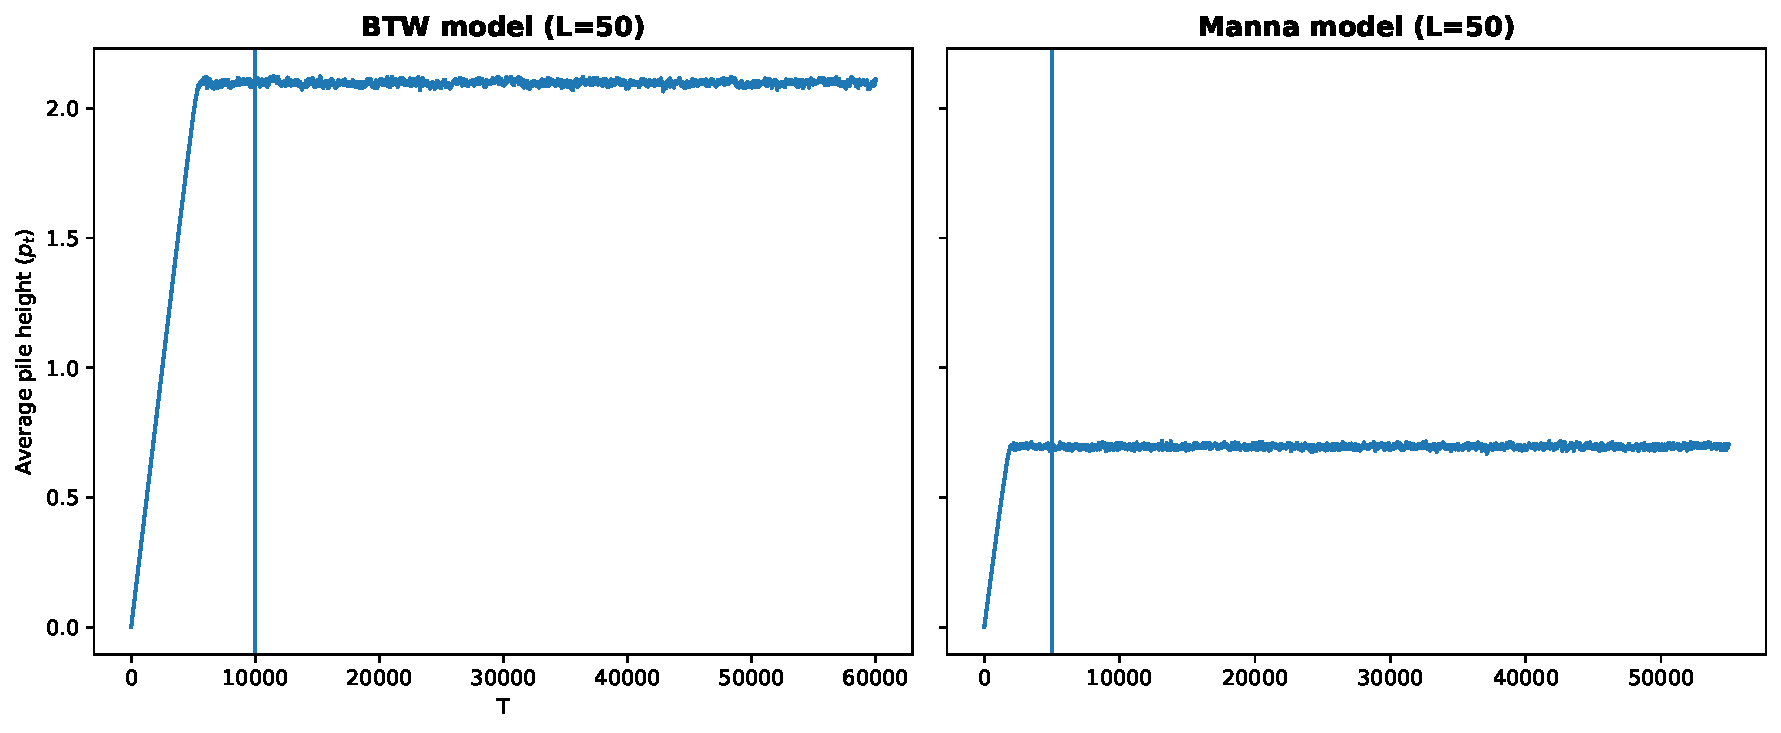
\includegraphics[width=0.80\linewidth]{figures/average_height.pdf}
    \caption{Mean pile height at each time step for the
    BTW and Manna models with $L=50$. The vertical lines indicate the
    burn-in periods used in the subsequent analysis.}
    \label{fig:average-height}
\end{figure}

\subsection{Implementation}

The simulations and statistical analyses were implemented in Python and are provided in the submitted Jupyter notebook. Each sand pile was represented by an $L\times L$ integer-valued NumPy array. NumPy was used for numerical operations and pseudorandom number generation, Sklearn for computing $R^2$, Pandas for correlation, and Matplotlib for visualisation. A fixed random seed \texttt{12345} was used to make the simulations reproducible.\\

To perform an avalanche, an initial implementation searched the full lattice for unstable sites. However, this $O(L^2)$ algorithm became very computational expensive especially for larger $L$ values. Hence this was later replaced using a first-in, first-out queue with Python's \texttt{collections.deque}, which supports append and removal operations in approximately $O(1)$ \cite{PythonDeque}. Only sites whose heights could have changed were added to the queue, avoiding repeated full-lattice searches and improving the efficiency of the simulation.

\section{Avalanche properties}\label{sec:properties}
%Topples, Area, Loss and Length
% average height and correlations if include

In this report, we investigate four avalanche properties:
\begin{enumerate}
    \item \textbf{Topples}. The number of topples required to take the system back to a stable configuration;
    \item \textbf{Area.} The number of unique sites that have been toppled;
    \item \textbf{Loss.} The number of grains dissipate off the open boundaries;
    \item \textbf{Length.} The maximum $L_1$-distance from the avalanche origin $(x_0, y_0)$ where the sand is dropped, to any toppled sites.
    \[
    L=\max_{(x,y) \in A}\{|x_0-x|+|y_0-y|\}
    \]where $A$ are the sites that has been toppled.

\end{enumerate}

$L_1$ distance gives us an intuitive interpretation of length as it measures the minimum number of lattice steps between an avalanche origin and a toppled site (since we only move in vertical or horizontal directions). Note that this simpler definition differs from the ``radius of gyration" previously discussed in Chapter \ref{ch:introduction}.\\

% Q8 here
Positive associations are expected between topples, area, length and possibly loss, since an avalanche having more topplings is more likely to affect more unique sites and propagate further from its origin. Associations with loss may be weaker since dissipation only happens when an avalanche reaches the open boundary. To examine this, we calculate pairwise Spearman rank correlations between all four properties. Spearman correlation \cite{Spearman1904} was selected because it measures monotonic association and is less sensitive than Pearson correlation to the extreme observations produced by heavy-tailed distributions.

\section{Empirical distribution}\label{sec:empirical}

% positive observations, PMF and log binnin
Many sand drops produce no avalanches. Power-law analysis is therefore restricted to positive observations since $\log x$ is undefined at $x=0$. However, we did not exclude zero values simply due to this reason. For topples and area, a zero value indicates that no avalanche occurred, hence it makes natural sense to examine its positive distribution. Meanwhile, a zero length may also represent an avalanche confined to its origin, and a zero loss indicates no boundary dissipation whether or not an avalanche has happened. Hence, we report $P(X=0)$ separately for loss and length.\\

For visual clarity when comparing across different system sizes, the empirical distributions were displayed using 30 logarithmically spaced bins. Log binning was used only for visualisation and the cutoff selection and fitted exponents were performed from other methods. This prevents the estimated exponents from depending on the selected number of bins.

\section{Power law fitting}\label{sec:powerlaw}

% survival function, cutoff selection
Throughout this report, $\log$ denotes the natural log. To identify an approximate power-law region, we first calculate the survival function $S(x)=P(X\geq x)$. This is smoother than our empirical PMF, making the departure from an approximately straight region easier to identify. For each candidate upper cutoff, a straight line was fitted to $\log S(x)$ against $\log x$ using observations up to that cutoff. The largest candidate satisfying the chosen $R^2$ threshold was selected. We used $R^2 \geq 0.95$ for topples and area and $R^2 \geq 0.88$ for length. The threshold was lowered for length to ensure the selected fitting region contained enough points. These thresholds only serves as practical criteria for identifying approximately linear regions of a power-law distribution.\\

%raw pmf fitting region, collapse, common exponent across L
Theoretically, for an untruncated power law, we have,
\[
P(x) \propto x^{-\tau}
\]
And the survival function should therefore asymptotically satisfy
\[
S(x)=P(X\geq x) \propto x^{1-\tau}
\]
Nevertheless, in our finite system, the survival function may deviate from this ideal asymptotic relationship due to discreteness of observables $x$, their finite and relatively small range, as well as the upper tail truncation. Therefore the survival function slope was used only to select the cutoff and was not reported as the final exponent.\\

After cutoff selection, a common exponent was estimated directly from the unbinned empirical PMF values within the selected scaling regions. Values from all system sizes were pooled and fitted by ordinary least squares (OLS) in log-log space:
\[
\log P(x) = -\tau_x \log(x)+C
\]
This produced a common exponent $\tau$ describing the family of finite size distributions. For the Manna model, values below the first non-plateau log bin were excluded as a lower cutoff. Nevertheless, note that the estimated exponent remains sensitive to the selected upper cutoff. If the cutoff extends into the sparse finite-size tail, tail observations can influence the fitted slope. This limitation will be discussed further in Chapter~\ref{ch:discussion}.\\

% finite size scaling: log N scaling, refit, RMSE and maximum deviation
To investigate the log finite size correction as proposed by Yadav et al.  \cite{Yadav2022FiniteSize}, the probability distributions are rescaled by $\log N$ where $N=L^2$. Hence the rescaled response variable becomes
\[
\log (\log (N)P(x))=\log P(x)+\log\log N
\]
A new common fit was then calculated, $\tau'$:
\[
 \log (\log (N)P(x))= -\tau_x' \log(x)+C'
\]
The quality of the common collapse was compared before and after
rescaling using the overall RMSE and maximum residual in log scale. Smaller values indicate that the curves agree closer to their common fitted line.

\section{Exponential fitting}\label{sec:exponential}

% P(X=0), positive component distribution, semilog fit, R^2, RMSE, residual
Exponential distributions were considered for the loss and length. $P(X=0)$ is reported separately for both properties and a log-linear model is fitted to the empirical probabilites for $x>0$ values.
\[
\log P(x) = -\lambda x +C
\]
Here, $\lambda$ corresponds to the decay rate. The larger the value, the faster the decay.\\

We use $R^2$ value and RMSE values to examine the fit and use residual plots for diagnosing systematic patterns. In particular, curvature or an S-shaped residual pattern indicates that a single exponential decay rate may not adequately describe the observed distribution.
